\documentclass{article}
\usepackage[usenames,dvipsnames]{xcolor}
\usepackage{array}
\usepackage{minted}
\usepackage{float}
\usepackage{amsmath}
\usepackage{color}
\usepackage{graphicx}
\usepackage[utf8]{inputenc}
\usepackage[T1]{fontenc}
\usepackage[english]{babel}
\usepackage[makeroom]{cancel}

\definecolor{bg}{rgb}{0.95,0.95,0.95}

\begin{document}
\title{\textbf{''Introduction to Artificial Intelligence: Homework \#5''}}
\author{LAINE Bastien \#20156441}
\date{Nov. 18th 2015}
\maketitle
\tableofcontents

\newpage
    \section{Problem 1}
        \subsection{A}
            \subsubsection{$p(a,b)\ne p(a).p(b)$?}
                Using the formula $p(a, b)=\sum_c p(a, b, c)$, we can compute $p(a, b)$
                \[
                    \begin{tabular}{|c|c|c|}
                        \hline
                        $a$&$b$&$p(a,b)$\\
                        \hline
                        0&0&0.336\\
                        \hline
                        0&1&0.264\\
                        \hline
                        1&0&0.256\\
                        \hline
                        1&1&0.144\\
                        \hline
                    \end{tabular}
                \]
                According to the same formula, we can draw that $p(a)=\sum_b p(a,b)$ and that $p(b)=\sum_a p(a,b)$

                \[
                    \begin{tabular}{|c|c|}
                        \hline
                        a&p(a)\\
                        \hline
                        0&0.600\\
                        \hline
                        1&0.400\\
                        \hline
                    \end{tabular}
                \]
                \[
                    \begin{tabular}{|c|c|}
                        \hline
                        b&p(b)\\
                        \hline
                        0&0.592\\
                        \hline
                        1&0.408\\
                        \hline
                    \end{tabular}
                \]
                \[
                    \begin{tabular}{|c|c|c|}
                        \hline
                        $a$&$b$&$p(a)p(b)$\\
                        \hline
                        0&0&0.355\\
                        \hline
                        0&1&0.244\\
                        \hline
                        1&0&0.236\\
                        \hline
                        1&1&0.163\\
                        \hline
                    \end{tabular}
                \]
                Given that, we can clearly saw that $p(a, b)\ne p(a).p(b)$
            \subsubsection{$p(a,b|c)=p(a|c)p(b|c)$?}
        \subsection{B}
            \subsubsection{p(a)}
            \subsubsection{p(b|c)}
            \subsubsection{p(c|a)}
            \subsubsection{p(a,b,c)=p(a)p(c|a)p(b|c)?}
                Using Bayes formula, we can easily deduct that:
                \[
                    \begin{array}{rcl}
                        p(a)p(c|a)p(b|c) &=& p(a\cap c)p(b|c)\\
                        &=& p(a\cap c\cap b)\\
                        p(a)p(c|a)p(b|c) &=& p(a, b, c)\\
                    \end{array}
                \]
                Finaly, we can say that $p(a,b,c)=p(a)p(c|a)p(b|c)$
            \subsubsection{Directed graph}
    \section{Problem 2}
        \subsection{A}
            We begin with the whole set of example.\\
            First, we compute the entropy of this step using the formula:
            \[
                \sum_{i\in\{0, 1\}} -p_i.\log_2(p_i)
            \]
            Then, we'll try to divide our set according to each input.\\
            Once done, we compute the average entropy of the 2 new set by ponderating both entropy by their Cardinality over the parent's cardinality.\\
            then, we choose the ``most interesting split'', that is to say the one whose entropy is maximum.\\

            Then, we compute again this step, but for our two new sub set. We'll stop our iteration when we found a leaf, that is to say a state where all of the ``outputs'' are the same (either 0 or 1 in our case)\\
            Since such a process is boring, I've developed a Bash script, whose goal is to create the graph. Executing it generate a PlantUML file. (Dependencie: bc)\\

            Finaly, the final result is the following:
            \begin{figure}[H]
                \centering
                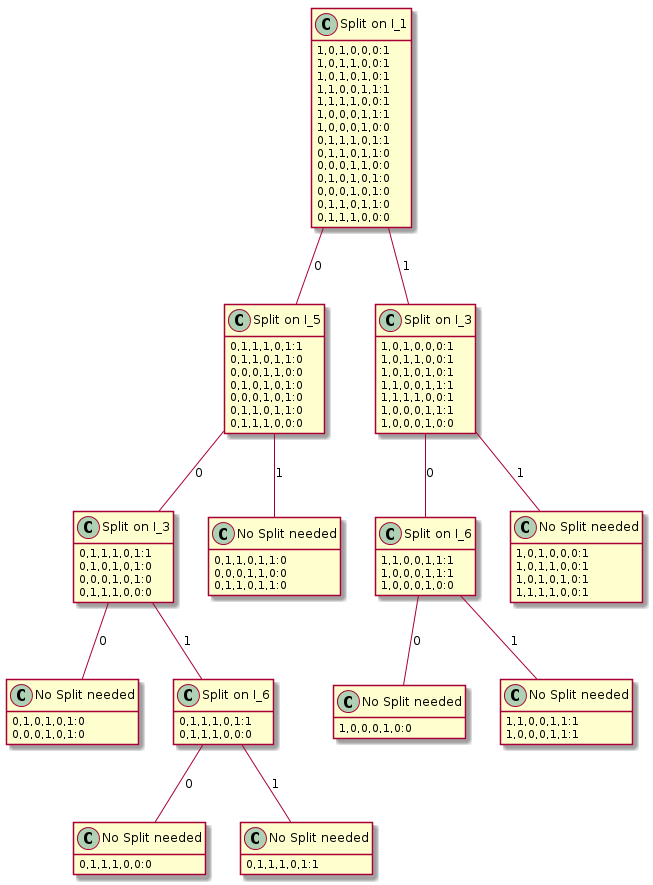
\includegraphics[scale=0.5]{problem2/graph.png}
                \caption{Final decision tree}
            \end{figure}


    \section{Problem 3}
        \subsection{A}
    \section{Problem 4}
        \subsection{A}
            Here is a copy of the sigmoid function you can find on ``problem4/mnist.py''\\
            I use the Numpy's exponential, because it allows me to calculate the exp of every term of an array.
            \begin{minted}[linenos]{python}
def sigmoid(x):
    # a sigmoid of x

    # [4.A] FILL YOUR CODE HERE
    return 1/(1+np.exp(-x))
            \end{minted}
        \subsection{B}
            Here is a copy of the propagate function you can find on ``problem4/mnist.py''\\
            \begin{minted}[linenos]{python}
def propagate(x):
    # propagate an input x to the output layer

    # [4.B] FILL YOUR CODE HERE

    #Copy data to the input layer
    np.copyto(layers[0], x)

    #Compute y for the hidden layer
    layers[1]=sigmoid(np.dot(layers[0], weights[0]))

    #Compute y for the output layer
    layers[2]=sigmoid(np.dot(layers[1], weights[1]))

    return layers[2]
            \end{minted}
        \subsection{C}
            Here is a copy of the backpropagate function you can find on ``problem4/mnist.py''\\
            \begin{minted}[linenos]{python}
def backpropagate(y_true, learning_rate):
    # backpropagate an error from the output layer and update weights

    # [4.C] FILL YOUR CODE HERE

    #Compute deltas for output layer
    outerr = layers[2]*(1-layers[2])*(y_true-layers[2]) #(1, 10)

    #Compute deltas for hidden layers
    hiddenerr = layers[1]*(1-layers[1])*(outerr.dot(weights[1].T)) #(1, 50)

    #Change hidden-output weigths
    weights[1] = weights[1] + learning_rate*layers[1].T.dot(outerr) #(50, 10)

    #Change input-hidden weigths
    weights[0] = weights[0] + learning_rate*layers[0].T.dot(hiddenerr) #(784, 50)
            \end{minted}
        \subsection{D}
            \begin{tabular}{|c|c|}
                \hline
                Interation & Error \\
                \hline
                0 & 0.537155024662484 \\
                \hline
                1000 & 0.149062349319850 \\
                \hline
                2000 & 0.124576012748911 \\
                \hline
                3000 & 0.111371770213344 \\
                \hline
                $\cdots$ & $\cdots$\\
                \hline
                40000 & 0.042501735109164 \\
                \hline
                41000 & 0.041759621834425 \\
                \hline
                42000 & 0.040796208555681 \\
                \hline
                43000 & 0.042767219131763 \\
                \hline
                44000 & 0.041207886314534 \\
                \hline
                45000 & 0.040088629855188 \\
                \hline
                46000 & 0.039915601152924 \\
                \hline
                47000 & 0.040204314440399 \\
                \hline
                48000 & 0.039018303138219 \\
                \hline
                49000 & 0.038433948782109 \\
                \hline
                Validation data & 0.038829476442797\\
                \hline
                Test data & 0.039398346519943\\
                \hline
            \end{tabular}
        \subsection{E}
\end{document}
